\chapter{Tools di analisi}
lorem ipsum lorem ipsum
\section{DDSFuzz}
DDSFuzz è un tool di analisi open source con l'obiettivo di 
effettuare test di tipo fuzz
in modo da testare vari input che il middleware DDS può
ricevere durante la sua esecuzione. Prima di questo strumento 
non esistevano (o non erano disponibili al pubblico) soluzioni
per effettuare questo tipo di test specifico per il DDS, mancanza
che questo tool cerca di colmare. Infatti anche se esistono tool 
come RoboFuzz e Deng, quest'ultimi vengono utilizzati solamente
per testare applicativi ROS (Robotic Operation System), che 
utilizzano solo una parte delle funzioni del DDS, tralasciando
così delle funzionalità del middleware che non vengono usufruite
da ROS \cite{10.1145/3691620.3695073}.


\subsection{Fuzz testing}
Prima di parlare del tool DDSFuzz dobbiamo prima comprendere 
il significato di fuzzing (chiamato anche fuzz test) che è
alla base del funzionamento di questo tool. Il fuzzing è un test
automatizzato che serve a trovare e creare casi limite utilizzando
dati di input invalidi in modo tale da esplorare più vulnerabilità
possibili all'interno di un software. 
Inizialmente i primi tool di fuzzing non erano molto 
semplici da utilizzare o conosciuti, ma con il tempo questi strumenti
sono migliorati rendendoli più user-friendly aumentando così la 
loro frequenza di uso per testare software. Quest'ultimi possono
essere sottoposti a questo tipo di test possono essere 
di ogni tipo: compilatori, applicazioni, protocolli network 
e kernel \cite{8371326}.

\begin{figure}[H]
    \centering
    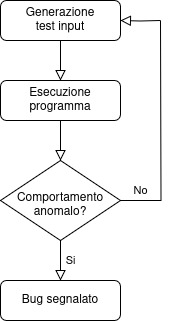
\includegraphics[width=5cm, keepaspectratio]{img/Diagramma di flusso fuzzer.jpg}
    \caption{Diagramma di flusso del funzionamento di un fuzzer.}
    \label{funzionamento fuzzer}
\end{figure}

Questi fuzzing test simulano un attacco mandando al software
che si vuole testare input regolari e irregolari, 
in modo tale da poter 
accedere ad ogni parte del codice con ogni tipo di input possibile.
In questo modo è possibile analizzare il comportamento del software
ed è possibile distinguere casi anomali o insicuri che non dovrebbero
essere possibili. Infatti quando questo test è attivo il fuzzer riceverà
varie informazioni riguardanti lo stato e l'output del programma, in 
modo tale da poter distinguere il suo comportamento. Se viene scoperto
qualche comportamento anomalo (ad esempio un segmentation fault) il 
fuzzer segnalerà in un log gli input utilizzati in modo tale da poter 
segnalare il bug.

Tuttavia dato che questi test sono generalizzati per essere compatibili
con vari software, si crea una sorta di imprecisione nel mandare i vari 
input. Questi input a volte non sono variegati a sufficienza 
per analizzare ogni singola parte del software che stiamo analizzando.
Inoltre in molti casi può anche succedere che vengono creati
dei test che non sono necessari consumando risorse e tempo inutilmente.

Per migliorare la qualità di questi test è stato 
creato il DDSFuzz che essendo un fuzzer specifico solamente per 
il middleware DDS rimuove molte delle imprecisioni di un fuzzer 
più generico.

\subsection{Punti di forza di DDSFuzz}
DDSFuzz essendo specializzato per il DDS prende in considerazione 
molte sue caratteristiche che non sono presenti in altri software
o protocolli. La prima considerazione che viene 
effettuata da DDSFuzz che avviene durante l'esecuzione del middleware DDS è
la topologia della rete che può mutare nel tempo creando problemi per i
fuzzer tradizionali che non si adattano ai suoi cambiamenti. Infatti certi
dispositivi si possono connettere o disconnettere dalla rete a loro 
piacimento rendendo quindi necessario cambiare i destinatari 
degli input di test 
evitando ad esempio di trasmettere informazioni verso un'entità 
che si è disconnessa e quindi impossibilitata a ricevere ulteriori
aggiornamenti. DDSFuzz prende anche in considerazione le
policy QoS e 
le funzionalità abilitate dal DDS security, come
l'autenticazione e il controllo accessi, in modo tale da
poter creare test più accurati. 

Finita l'esecuzione di DDSFuzz ci ritroviamo con due tipologie
di bug che possiamo riscontrare in un applicativo DDS:
\begin{itemize}
    \item BUG TRADIZIONALI: racchiude tutti i classici bug 
    che sono presenti anche in altri software, un esempio può 
    essere un buffer overflow;
    \item BUG SEMANTICI: questo bug avviene quando viene violata
    una norma definita dallo standard DDS, come 
    ad esempio un bypass dell'autenticazione. 
    Dato che il loro comportamento
    non è facilmente categorizzabile risulta più difficile individuarli;
\end{itemize}
Uno dei maggiori punti di forza di DDSFuzz sta proprio nel trovare
questi bug semantici, quasi impossibili da identificare per gli altri 
fuzzer. Durante l'esecuzione di DDSFuzz vengono eseguite in parallelo 
tre implementazioni (Fast DDS \cite{FastDDS}, Cyclone DDS \cite{CycloneDDS}, 
OpenDDS \cite{OpenDDS1}) vendor 
del DDS in modo tale da identificare
se i risultati dei test input rimangono consistenti tra di loro in 
ognuna delle esecuzioni. 
Se otteniamo una soluzione differente in una sola 
delle implementazioni utilizzate possiamo dire che quest'ultima ha un 
comportamento anomalo generato da un bug di tipo semantico 
\cite{10.1145/3691620.3695073}. 

\subsection{Composizione di DDSFuzz}
DDSFuzz è composto da tre elementi principali chiamati: 
DDS input generator, DDS program executor e bug detector.
\begin{itemize}
    \item DDS INPUT GENERATOR: Si occupa di generare degli input 
    specifici per il DDS prendendo in considerazione la topologia
    della rete, delle policy QoS e dei parametri di sicurezza del 
    DDS security. In questo modo non vengono generati test inutili 
    che non servono per l'analisi dell'esecuzione. 
    Questi test poi successivamente vengono adattati per essere 
    compatibili con il 
    protocollo RTPS in modo tale che il DDS program executor utilizzare 
    immediatamente questi input generati;
    \item DDS PROGRAM EXECUTOR: ricevuti gli input generati 
    li invierà alle
    tre implementazioni del DDS, mandando feedback  al DDS input generator
    sulla validità e efficacia dei test generati;
    \item BUG DETECTOR: a differenza di altri bug detector provenienti da 
    fuzzer tool generici, quest'ultimo riesce a distinguere tra bug 
    di tipo tradizionale e bug semantici, grazie all'analisi
    degli output delle implementazioni del DDS
    \cite{10.1145/3691620.3695073};
\end{itemize}